\documentclass[10pt]{article}
\usepackage{graphicx}
\usepackage[margin=1.5cm]{geometry}
\usepackage{amsmath}
\def\brcurs{{\mbox{$\resizebox{.16in}{.08in}{
\includegraphics{BoldR}}$}}}
\def\rcurs{{\mbox{$\resizebox{.16in}{.08in}{
\includegraphics{ScriptR}}$}}}

\begin{document}
\twocolumn

\title{Thursday Warm-up: Potentials}
\author{Prof. Jordan C. Hanson}

\maketitle

\section{Memory Bank}

\begin{itemize}
\item \textbf{Fourier series} for a function $f(x)$:
\begin{align}
f(x) &= \frac{A_0}{2} + \sum_{n=1}^{\infty} \left(A_n \cos nx + B_n \sin nx \right) \label{eq:1} \\
A_n &= \frac{1}{\pi}\int_0^{2\pi} f(x) \cos (nx) dx ~~ (n=0,1,2,...) \label{eq:2} \\
B_n &= \frac{1}{\pi}\int_0^{2\pi} f(x) \sin (nx) dx ~~ (n=1,2,...) \label{eq:3}
\end{align}
\item Laplace's equation in 2D Cartesian coordinates:
\begin{equation}
\frac{\partial^2 X}{\partial x^2} + \frac{\partial^2 Y}{\partial y^2} = 0
\end{equation}
\end{itemize}

\begin{figure}
\centering
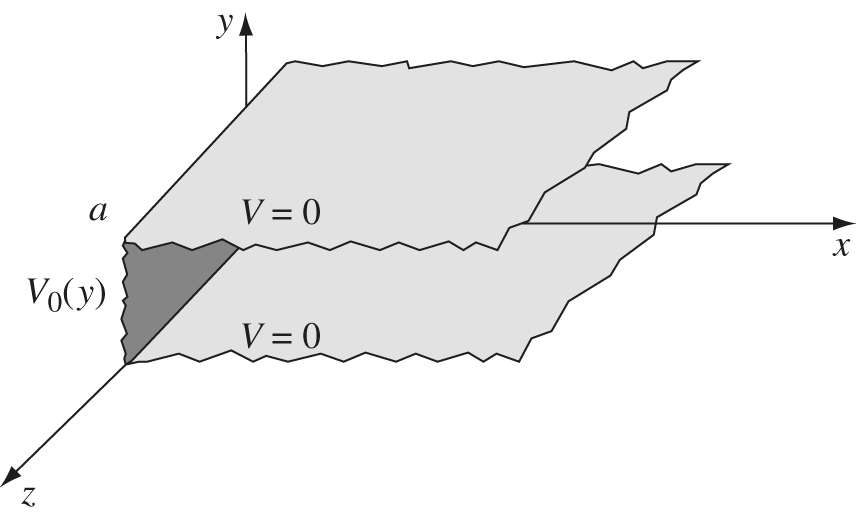
\includegraphics[width=0.35\textwidth]{figures/3_17.jpg}
\caption{\label{fig:1} An infinite ``slot'' in the xy-plane, defined by two grounded conductors in the xz-plane separated by a distance $a$, with boundary condition $V_0(y)$ in the yz-plane.}
\end{figure}

\section{Separation of Variables}

\begin{enumerate}
\item \textbf{Fourier Series}.  Suppose a function is $f(x)=x$ between 0 and $2\pi$, and then $f(x) = (x-2\pi)$ from $2\pi$ to $4\pi$, and then $f(x) = (x-4\pi)$ from $4\pi$ to $6\pi$, ..., repeating periodically.  (a) Develop the \textit{Fourier series} for $f(x)$ by computing the coefficients $A_n$ and $B_n$ using equations in the Memory Bank.  (b) Equations \ref{eq:2} and \ref{eq:3} impose \textit{boundary conditions} that build Eq. \ref{eq:1}. (c) Using software, plot the series up to $n=5$. \\ \vspace{5cm}
\item Two infinite grounded metal plates lie parallel to the xz plane, one at $y=0$, and the other at $y=a$ (Fig. \ref{fig:1}).  The left end, at $x=0$, is closed off with an infinite strip insulated from the two plates, and maintained at a voltage $V_0(y)$.  Find the voltage inside the slot.
\begin{itemize}
\item Write down \textit{four} boundary values as equations. \\ \vspace{0.5cm}
\item Let the solution be \textit{separable}:
\begin{equation}
V(x,y) = X(x) Y(y)
\end{equation}
Substitute this into the 2D version of Laplace's equation in Cartesian coordinates, and separate the $X$ and $Y$ portions into distinct terms. \\ \vspace{1cm}
\item Argue that each term should be a \textit{constant}, for if (for example) $y$ is held constant and $x$ is varied, the left side of the equation would vary, while the right side would be constant at 0.
\item Since the $X$ constant and $Y$ constant are equal and opposite, set the $X$ constant to $k^2$ and the $Y$ constant to $-k^2$.  Try to guess the solutions for the separated equations for $X(x)$ and $Y(y)$. \\ \vspace{2cm}
\item Impose the boundary conditions for $x\neq 0$, and write an example solution for $V(x,y)$. \\ \vspace{2cm}
\item Laplace's equation admits \textit{linear combinations} of solutions: $V = a_1 V_1 + a_2 V_2 + ...$.  Write a series of solutions based on your example solution.
\end{itemize}
\end{enumerate}

\end{document}
